\documentclass[14pt]{extbook}
\usepackage{multicol, enumerate, enumitem, hyperref, color, soul, setspace, parskip, fancyhdr} %General Packages
\usepackage{amssymb, amsthm, amsmath, bbm, latexsym, units, mathtools} %Math Packages
\everymath{\displaystyle} %All math in Display Style
% Packages with additional options
\usepackage[headsep=0.5cm,headheight=12pt, left=1 in,right= 1 in,top= 1 in,bottom= 1 in]{geometry}
\usepackage[usenames,dvipsnames]{xcolor}
\usepackage{dashrule}  % Package to use the command below to create lines between items
\newcommand{\litem}[1]{\item#1\hspace*{-1cm}\rule{\textwidth}{0.4pt}}
\pagestyle{fancy}
\lhead{Makeup Progress Quiz 3}
\chead{}
\rhead{Version B}
\lfoot{4315-3397}
\cfoot{}
\rfoot{Fall 2020}
\begin{document}

\begin{enumerate}
\litem{
Write the equation of the graph presented below in the form $f(x)=ax^2+bx+c$, assuming  $a=1$ or $a=-1$. Then, choose the intervals that $a, b,$ and $c$ belong to.
\begin{center}
    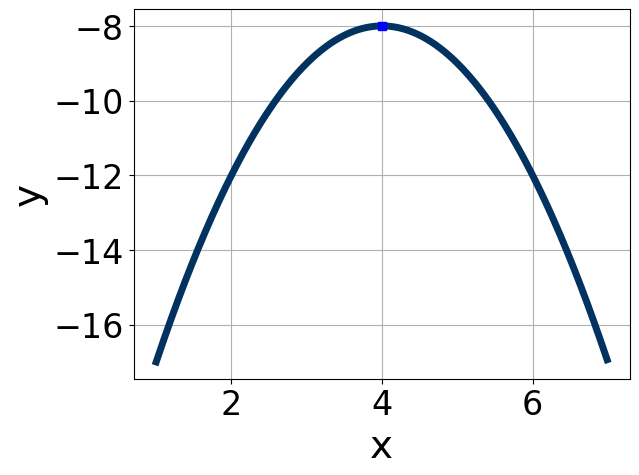
\includegraphics[width=0.5\textwidth]{../Figures/quadraticGraphToEquationB.png}
\end{center}
\begin{enumerate}[label=\Alph*.]
\item \( a \in [-1.9, -0.7], \hspace*{5mm} b \in [-9, -7], \text{ and } \hspace*{5mm} c \in [-11, -7] \)
\item \( a \in [0.5, 2.7], \hspace*{5mm} b \in [-9, -7], \text{ and } \hspace*{5mm} c \in [8, 10] \)
\item \( a \in [0.5, 2.7], \hspace*{5mm} b \in [7, 9], \text{ and } \hspace*{5mm} c \in [8, 10] \)
\item \( a \in [-1.9, -0.7], \hspace*{5mm} b \in [7, 9], \text{ and } \hspace*{5mm} c \in [-24, -23] \)
\item \( a \in [-1.9, -0.7], \hspace*{5mm} b \in [-9, -7], \text{ and } \hspace*{5mm} c \in [-24, -23] \)

\end{enumerate} }
\litem{
Solve the quadratic equation below. Then, choose the intervals that the solutions belong to, with $x_1 \leq x_2$ (if they exist).\[ -19x^{2} -7 x + 4 = 0 \]\begin{enumerate}[label=\Alph*.]
\item \( x_1 \in [-0.54, -0.25] \text{ and } x_2 \in [0.33, 1.18] \)
\item \( x_1 \in [-6.11, -5.58] \text{ and } x_2 \in [11.82, 13.16] \)
\item \( x_1 \in [-1.23, -0.64] \text{ and } x_2 \in [-0.1, 0.64] \)
\item \( x_1 \in [-19.5, -18.77] \text{ and } x_2 \in [18.17, 18.65] \)
\item \( \text{There are no Real solutions.} \)

\end{enumerate} }
\litem{
Factor the quadratic below. Then, choose the intervals that contain the constants in the form $(ax+b)(cx+d); b \leq d.$\[ 36x^{2} +7 x -15 \]\begin{enumerate}[label=\Alph*.]
\item \( a \in [20, 29], \hspace*{5mm} b \in [-14, -3], \hspace*{5mm} c \in [0, 2], \text{ and } \hspace*{5mm} d \in [3, 10] \)
\item \( a \in [6, 14], \hspace*{5mm} b \in [-14, -3], \hspace*{5mm} c \in [4, 6], \text{ and } \hspace*{5mm} d \in [3, 10] \)
\item \( a \in [3, 6], \hspace*{5mm} b \in [-14, -3], \hspace*{5mm} c \in [7, 13], \text{ and } \hspace*{5mm} d \in [3, 10] \)
\item \( a \in [-2, 2], \hspace*{5mm} b \in [-26, -13], \hspace*{5mm} c \in [0, 2], \text{ and } \hspace*{5mm} d \in [20, 35] \)
\item \( \text{None of the above.} \)

\end{enumerate} }
\litem{
Solve the quadratic equation below. Then, choose the intervals that the solutions belong to, with $x_1 \leq x_2$ (if they exist).\[ 17x^{2} -12 x + 2 = 0 \]\begin{enumerate}[label=\Alph*.]
\item \( x_1 \in [-2.72, -2.13] \text{ and } x_2 \in [2.87, 3.19] \)
\item \( x_1 \in [-0.87, -0.05] \text{ and } x_2 \in [-0.29, 0.2] \)
\item \( x_1 \in [4.43, 4.94] \text{ and } x_2 \in [6.92, 8.14] \)
\item \( x_1 \in [-0.06, 0.32] \text{ and } x_2 \in [-0.13, 0.86] \)
\item \( \text{There are no Real solutions.} \)

\end{enumerate} }
\litem{
Solve the quadratic equation below. Then, choose the intervals that the solutions $x_1$ and $x_2$ belong to, with $x_1 \leq x_2$.\[ 15x^{2} +7 x -36 = 0 \]\begin{enumerate}[label=\Alph*.]
\item \( x_1 \in [-9.4, -7.43] \text{ and } x_2 \in [-0.13, 0.5] \)
\item \( x_1 \in [-4.13, -3.08] \text{ and } x_2 \in [0.55, 0.75] \)
\item \( x_1 \in [-27.33, -25.94] \text{ and } x_2 \in [19.92, 20.04] \)
\item \( x_1 \in [-2.4, -1.57] \text{ and } x_2 \in [1.1, 1.79] \)
\item \( x_1 \in [-0.82, 0.12] \text{ and } x_2 \in [3.98, 4.46] \)

\end{enumerate} }
\litem{
Solve the quadratic equation below. Then, choose the intervals that the solutions $x_1$ and $x_2$ belong to, with $x_1 \leq x_2$.\[ 15x^{2} +38 x + 24 = 0 \]\begin{enumerate}[label=\Alph*.]
\item \( x_1 \in [-3.27, -2.6] \text{ and } x_2 \in [-0.62, -0.56] \)
\item \( x_1 \in [-6.19, -5.45] \text{ and } x_2 \in [-0.34, -0.23] \)
\item \( x_1 \in [-1.38, -0.87] \text{ and } x_2 \in [-1.33, -1.19] \)
\item \( x_1 \in [-20.19, -18.82] \text{ and } x_2 \in [-18.04, -17.94] \)
\item \( x_1 \in [-2.41, -1.51] \text{ and } x_2 \in [-0.69, -0.63] \)

\end{enumerate} }
\litem{
Graph the equation below.\[ f(x) = (x+4)^2 - 14 \]\begin{enumerate}[label=\Alph*.]
\begin{multicols}{2}\item 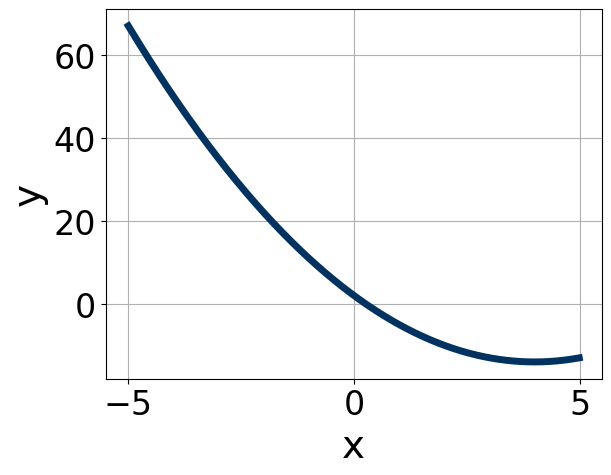
\includegraphics[width = 0.3\textwidth]{../Figures/quadraticEquationToGraphCopyAB.png}\item 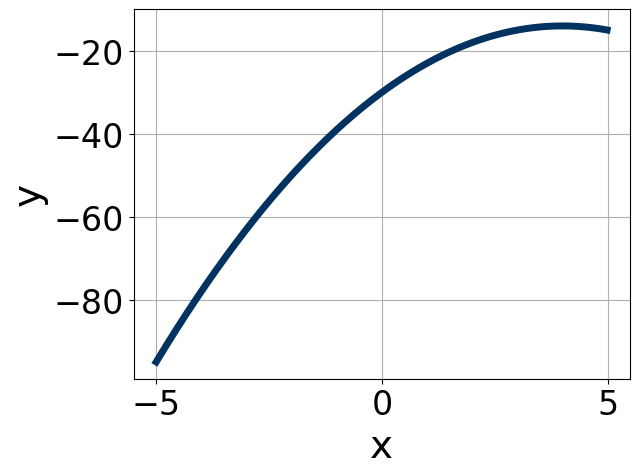
\includegraphics[width = 0.3\textwidth]{../Figures/quadraticEquationToGraphCopyBB.png}\item 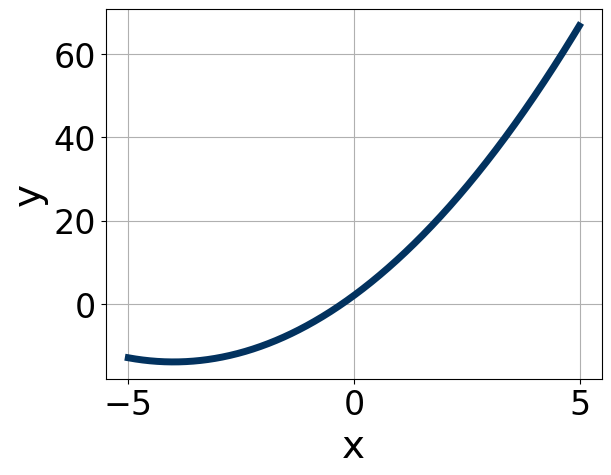
\includegraphics[width = 0.3\textwidth]{../Figures/quadraticEquationToGraphCopyCB.png}\item 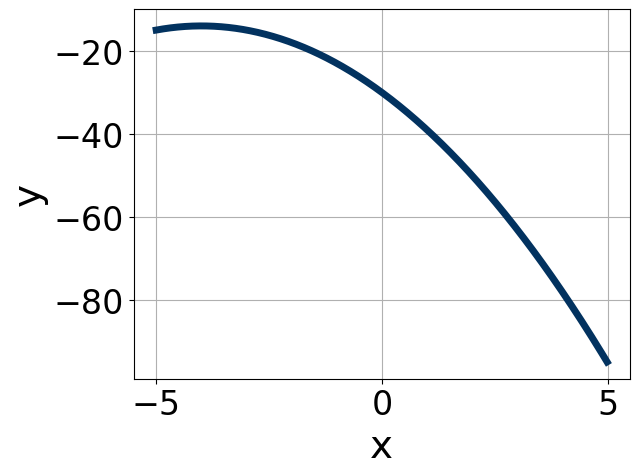
\includegraphics[width = 0.3\textwidth]{../Figures/quadraticEquationToGraphCopyDB.png}\end{multicols}\item None of the above.
\end{enumerate} }
\litem{
Factor the quadratic below. Then, choose the intervals that contain the constants in the form $(ax+b)(cx+d); b \leq d.$\[ 54x^{2} +15 x -25 \]\begin{enumerate}[label=\Alph*.]
\item \( a \in [2.8, 4.7], \hspace*{5mm} b \in [-5, 1], \hspace*{5mm} c \in [17.5, 18.9], \text{ and } \hspace*{5mm} d \in [3, 10] \)
\item \( a \in [0.6, 2.7], \hspace*{5mm} b \in [-30, -26], \hspace*{5mm} c \in [-1.5, 1.3], \text{ and } \hspace*{5mm} d \in [43, 48] \)
\item \( a \in [6.8, 10.1], \hspace*{5mm} b \in [-5, 1], \hspace*{5mm} c \in [4.1, 6.5], \text{ and } \hspace*{5mm} d \in [3, 10] \)
\item \( a \in [26, 27.8], \hspace*{5mm} b \in [-5, 1], \hspace*{5mm} c \in [1.4, 3.6], \text{ and } \hspace*{5mm} d \in [3, 10] \)
\item \( \text{None of the above.} \)

\end{enumerate} }
\litem{
Write the equation of the graph presented below in the form $f(x)=ax^2+bx+c$, assuming  $a=1$ or $a=-1$. Then, choose the intervals that $a, b,$ and $c$ belong to.
\begin{center}
    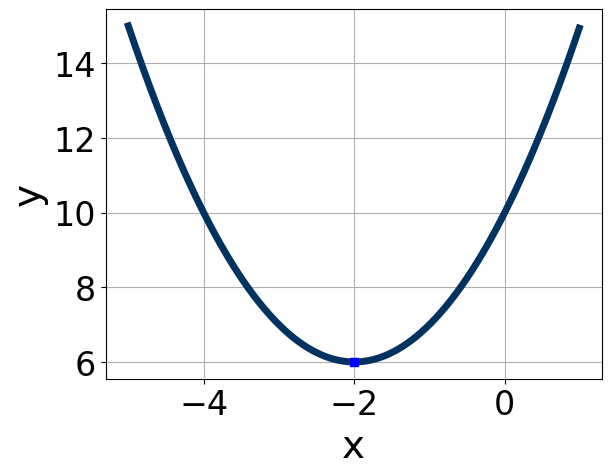
\includegraphics[width=0.5\textwidth]{../Figures/quadraticGraphToEquationCopyB.png}
\end{center}
\begin{enumerate}[label=\Alph*.]
\item \( a \in [1, 4], \hspace*{5mm} b \in [2, 7], \text{ and } \hspace*{5mm} c \in [7, 14] \)
\item \( a \in [-1, 0], \hspace*{5mm} b \in [2, 7], \text{ and } \hspace*{5mm} c \in [0, 5] \)
\item \( a \in [1, 4], \hspace*{5mm} b \in [-5, -2], \text{ and } \hspace*{5mm} c \in [-3, 1] \)
\item \( a \in [-1, 0], \hspace*{5mm} b \in [-5, -2], \text{ and } \hspace*{5mm} c \in [0, 5] \)
\item \( a \in [1, 4], \hspace*{5mm} b \in [-5, -2], \text{ and } \hspace*{5mm} c \in [7, 14] \)

\end{enumerate} }
\litem{
Graph the equation below.\[ f(x) = (x-3)^2 - 10 \]\begin{enumerate}[label=\Alph*.]
\begin{multicols}{2}\item 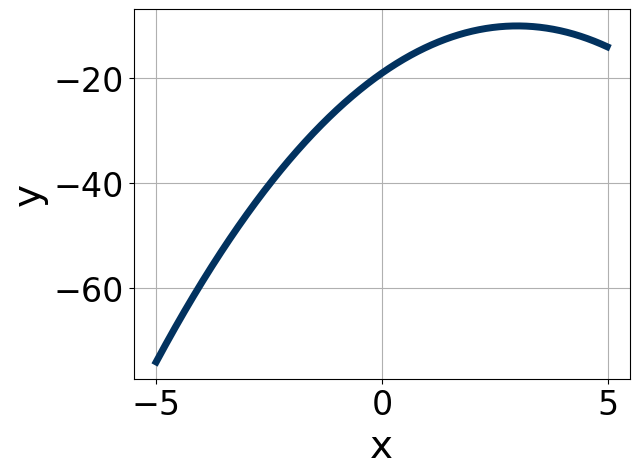
\includegraphics[width = 0.3\textwidth]{../Figures/quadraticEquationToGraphAB.png}\item 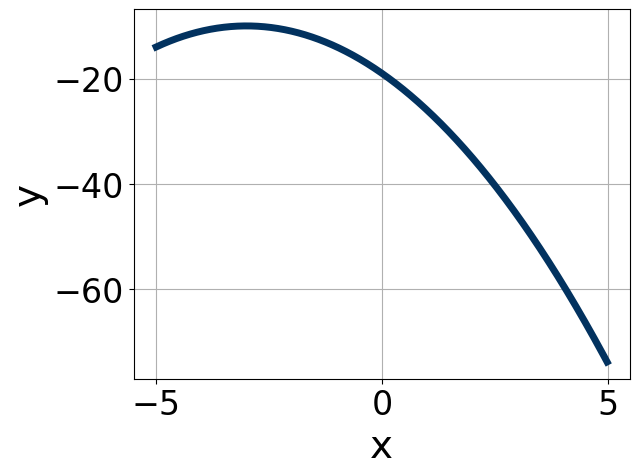
\includegraphics[width = 0.3\textwidth]{../Figures/quadraticEquationToGraphBB.png}\item 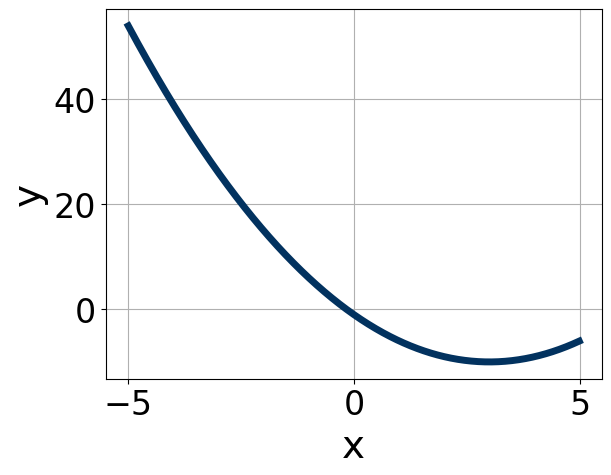
\includegraphics[width = 0.3\textwidth]{../Figures/quadraticEquationToGraphCB.png}\item 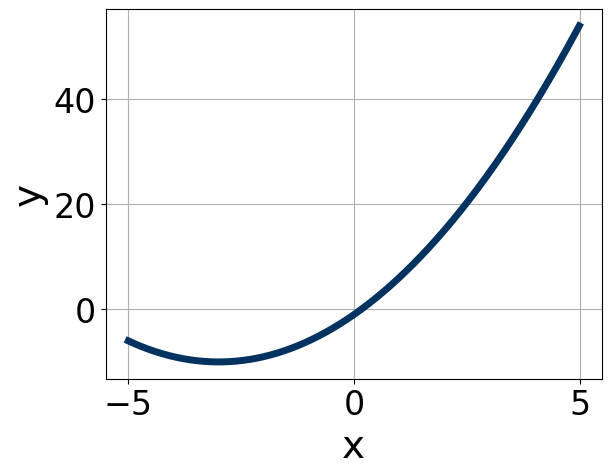
\includegraphics[width = 0.3\textwidth]{../Figures/quadraticEquationToGraphDB.png}\end{multicols}\item None of the above.
\end{enumerate} }
\end{enumerate}

\end{document}